\begin{figure}
\begin{center}
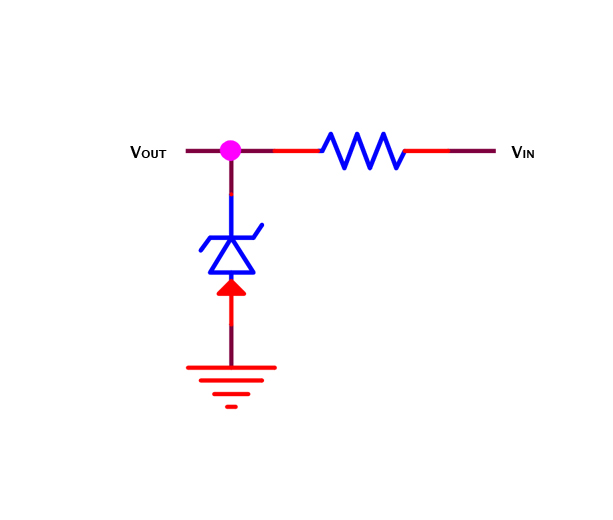
\includegraphics[width=8cm]{implementation/figures/GPIOprotection}
\end{center}
\caption{GPIO Pin Protection}
\label{fig:GPIOprotection}
\end{figure}


The Central Unit is controlled by a Raspberry Pi, and therefore the PCB for holding the ZigBee module is required to connect to the GPIO headers Raspberry Pi.  Initially it was thought that this could be done directly, however on further inspection it was discovered that the Raspberry Pi is very sensitive to signals above 50mA at 3.3v. It was decided to make a protection circuit for each of the GPIO pins that were in use. 

A simple protection circuit can be created using a resistor and Zener diode as seen in \textbf{Figure \ref{fig:GPIOprotection}}.  Zener diodes are much like other types of diodes in that it allows current to flow freely in one direction, however unlike other diodes if the voltage is above the 'breakdown' voltage it is allowed to flow as well. Using this property of Zener diodes a simple DC voltage regulator can be created when placed in series with a resistor, if the voltage coming into the system, \(V_{IN}\), is greater than the breakdown voltage of the Zener diode it flows to ground rather than to the GPIO pin. Therefore, a 3v3 Zener diode was used with a 330&\Omega& resistor. The resistor limits the current that goes into the Zener diode, protecting the overall circuit.

Due to the fact that the Raspberry Pi can only produce 50mA over the 3v3 pin, in order to power the XBee module that uses over close to 50mA when broadcasting, the 5v pin on the Raspberry Pi was need. This can provide up to 700mA although at 5v, this meant that a 3v3 voltage regulator was required to power the XBee module, this came in the form of an 'ST LD1117' which was available from the University of Glasgow Electrical Components Store. The 'ST LD1117' comes with a low drop out voltage of 1v therefore requiring a minimum supply of 4v. With the voltage regulator come the decoupling capacitors, as suggested by the supplied datasheet.

The pins between the Raspberry Pi and XBee module were connected as shown in table ~\ref{interfacePiXBee}.


\begin{center}
  \begin{tabular}{| l | l | l | l |}
    \hline
    \bf{Pin (Rapsberry Pi)} & \bf{Function (Rapsberry Pi)} & \bf{Pin (XBee)} & \bf{Function (XBee)} \\ \hline
     - & - & 1 & \(V_{CC}\) \\ \hline
	10 & \(Rx\) & 2 & \(D_{OUT}\) \\ \hline
	8 & \(Tx\) & 3 & \(D_{IN}\) \\ \hline
	12 & \(GPIO\) & 5 & \(Reset\) \\ \hline
	25 & \(GND\) & 10 & \(GND\) \\ \hline
	13 & \(GPIO\) & 12 & \(Sleep\) \\ \hline
	11 & \(GPIO\) & 13 & \(CTS\) \\ \hline
	7 & \(GPIO\) & 16 & \(RTS\) \\
    \hline
  \end{tabular}
\label{interfacePiXBee}\\
Figure ~\fig{interfaceARMXBee}: Connection between Raspberry Pi and XBee units
\end{center}


In addition to the pins required by the XBee module, three LEDs were placed on the Central Unit PCB. One LED is connected directly to the power supply showing that the board has power, the other two are connected to GPIO pins to be used for any purpose necessary.

As the Central Unit does not require a wireless power supply, using the standard USB power cable was acceptable and provides a constant 5v, 1000mA supply.
